% biography section
%
% If you have an EPS/PDF photo (graphicx package needed) extra braces are
% needed around the contents of the optional argument to biography to prevent
% the LaTeX parser from getting confused when it sees the complicated
% \includegraphics command within an optional argument. (You could create
% your own custom macro containing the \includegraphics command to make things
% simpler here.)
%
% or if you just want to reserve a space for a photo:

%\begin{IEEEbiography}[{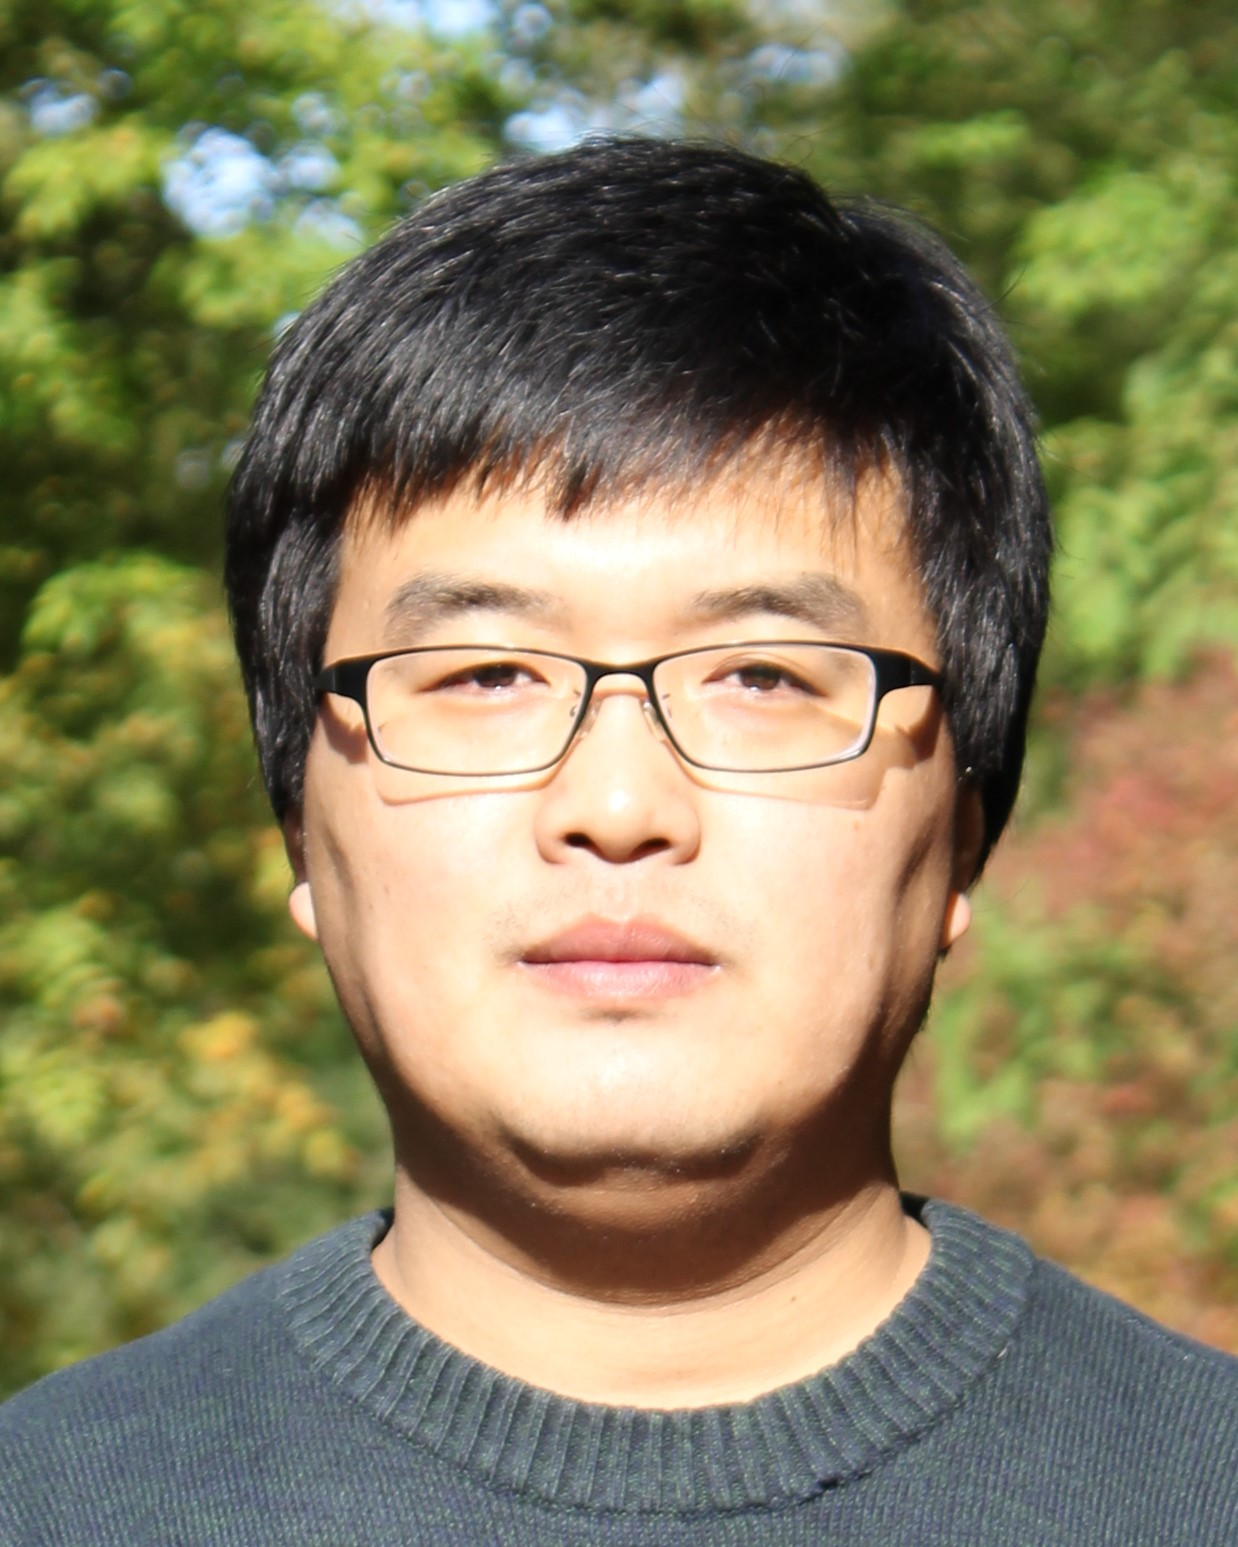
\includegraphics[width=1in,height=1.25in,clip,keepaspectratio]{figures/cui.jpg}}]{Ziqiang Cui}
%(M'13) received the M.Sc. and Ph.D. degrees from Tianjin University, China, in 2007 and 2009, respectively. He is currently an Associate Professor with the School of Electrical and Information Engineering, Tianjin University. His current research interests include electrical tomography instrumentation, signal processing, sensor design, and multi-phase flow measurement.
%\end{IEEEbiography}


\begin{IEEEbiography}[{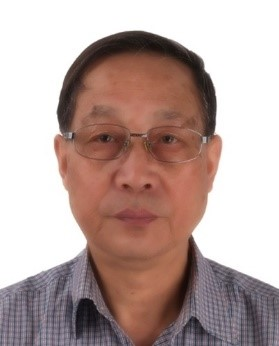
\includegraphics[width=1in,height=1.25in,clip,keepaspectratio]{figures/wang.jpg}}]{Huaxiang Wang}
(SM'06) received the degree from Tianjin University, China. He is currently a Professor with the School of Electrical and Information Engineering, Tianjin University.  His major research interests include sensing techniques and information processing, process parameter detection and control systems, and intelligent instrumentations.
\end{IEEEbiography}

% You can push biographies down or up by placing
% a \vfill before or after them. The appropriate
% use of \vfill depends on what kind of text is
% on the last page and whether or not the columns
% are being equalized.

\vfill

% Can be used to pull up biographies so that the bottom of the last one
% is flush with the other column.
%\enlargethispage{-5in}



% that's all folks 